
\documentclass[letterpaper,hide notes,xcolor={table,svgnames},pdftex,10pt]{beamer}
\def\showexamples{t}


%\usepackage[svgnames]{xcolor}

%% Demo talk
%\documentclass[letterpaper,notes=show]{beamer}

\usecolortheme{crane}
\setbeamertemplate{navigation symbols}{}

\usetheme{MyPittsburgh}
%\usetheme{Frankfurt}

%\usepackage{tipa}

\usepackage{hyperref}
\usepackage{graphicx,xspace}
\usepackage[normalem]{ulem}
\usepackage{multicol}
\usepackage{amsmath,amssymb,amsthm,graphicx,xspace}
\newcommand\SF[1]{$\bigstar$\footnote{SF: #1}}

\usepackage[default]{sourcesanspro}
\usepackage[T1]{fontenc}
\usepackage[scaled]{beramono}
\usepackage{tikzpagenodes}

\newcounter{tmpnumSlide}
\newcounter{tmpnumNote}


% old question code
%\newcommand\question[1]{{$\bigstar$ \small \onlySlide{2}{#1}}}
% \newcommand\nquestion[1]{\ifdefined \presentationonly \textcircled{?} \fi \note{\par{\Large \textbf{?}} #1}}
% \newcommand\nanswer[1]{\note{\par{\Large \textbf{A}} #1}}


 \newcommand\mnote[1]{%
   \addtocounter{tmpnumSlide}{1}
   \ifdefined\showcues {~\tiny\fbox{\arabic{tmpnumSlide}}}\fi
   \note{\setlength{\parskip}{1ex}\addtocounter{tmpnumNote}{1}\textbf{\Large \arabic{tmpnumNote}:} {#1\par}}}

\newcommand\mmnote[1]{\note{\setlength{\parskip}{1ex}#1\par}}

%\newcommand\mnote[2][]{\ifdefined\handoutwithnotes {~\tiny\fbox{#1}}\fi
% \note{\setlength{\parskip}{1ex}\textbf{\Large #1:} #2\par}}

%\newcommand\mnote[2][]{{\tiny\fbox{#1}} \note{\setlength{\parskip}{1ex}\textbf{\Large #1:} #2\par}}

\newcommand\mquestion[2]{{~\color{red}\fbox{?}}\note{\setlength{\parskip}{1ex}\par{\Large \textbf{?}} #1} \note{\setlength{\parskip}{1ex}\par{\Large \textbf{A}} #2\par}\ifdefined \presentationonly \pause \fi}

\newcommand\blackboard[1]{%
\ifdefined   \showblackboard
  {#1}
  \else {\begin{center} \fbox{\colorbox{blue!30}{%
         \begin{minipage}{.95\linewidth}%
           \hspace{\stretch{1}} Some space intentionally left blank; done at the blackboard.%
         \end{minipage}}}\end{center}}%
         \fi%
}



%\newcommand\q{\tikz \node[thick,color=black,shape=circle]{?};}
%\newcommand\q{\ifdefined \presentationonly \textcircled{?} \fi}

\usepackage{listings}
\lstset{basicstyle=\footnotesize\ttfamily,
	breaklines=true,
	aboveskip=15pt,
  	belowskip=15pt,
	frame=lines,
	numbers=left, basicstyle=\scriptsize, numberstyle=\tiny, stepnumber=0, numbersep=2pt
}

\usepackage{siunitx}
\newcommand\sius[1]{\num[group-separator = {,}]{#1}\si{\micro\second}}
\newcommand\sims[1]{\num[group-separator = {,}]{#1}\si{\milli\second}}
\newcommand\sins[1]{\num[group-separator = {,}]{#1}\si{\nano\second}}
\sisetup{group-separator = {,}, group-digits = true}

%% -------------------- tikz --------------------
\usepackage{tikz}
\usetikzlibrary{positioning}
\usetikzlibrary{arrows,backgrounds,automata,decorations.shapes,decorations.pathmorphing,decorations.markings,decorations.text,decorations.pathreplacing}

\tikzstyle{place}=[circle,draw=blue!50,fill=blue!20,thick, inner sep=0pt,minimum size=6mm]
\tikzstyle{transition}=[rectangle,draw=black!50,fill=black!20,thick, inner sep=0pt,minimum size=4mm]

\tikzstyle{block}=[rectangle,draw=black, thick, inner sep=5pt]
\tikzstyle{bullet}=[circle,draw=black, fill=black, thin, inner sep=2pt]

\tikzstyle{pre}=[<-,shorten <=1pt,>=stealth',semithick]
\tikzstyle{post}=[->,shorten >=1pt,>=stealth',semithick]
\tikzstyle{bi}=[<->,shorten >=1pt,shorten <=1pt, >=stealth',semithick]

\tikzstyle{mut}=[-,>=stealth',semithick]

\tikzstyle{treereset}=[dashed,->, shorten >=1pt,>=stealth',thin]

\usepackage{ifmtarg}
\usepackage{xifthen}
\makeatletter
% new counter to now which frame it is within the sequence
\newcounter{multiframecounter}
% initialize buffer for previously used frame title
\gdef\lastframetitle{\textit{undefined}}
% new environment for a multi-frame
\newenvironment{multiframe}[1][]{%
\ifthenelse{\isempty{#1}}{%
% if no frame title was set via optional parameter,
% only increase sequence counter by 1
\addtocounter{multiframecounter}{1}%
}{%
% new frame title has been provided, thus
% reset sequence counter to 1 and buffer frame title for later use
\setcounter{multiframecounter}{1}%
\gdef\lastframetitle{#1}%
}%
% start conventional frame environment and
% automatically set frame title followed by sequence counter
\begin{frame}%
\frametitle{\lastframetitle~{\normalfont(\arabic{multiframecounter})}}%
}{%
\end{frame}%
}
\makeatother

\makeatletter
\newdimen\tu@tmpa%
\newdimen\ydiffl%
\newdimen\xdiffl%
\newcommand\ydiff[2]{%
    \coordinate (tmpnamea) at (#1);%
    \coordinate (tmpnameb) at (#2);%
    \pgfextracty{\tu@tmpa}{\pgfpointanchor{tmpnamea}{center}}%
    \pgfextracty{\ydiffl}{\pgfpointanchor{tmpnameb}{center}}%
    \advance\ydiffl by -\tu@tmpa%
}
\newcommand\xdiff[2]{%
    \coordinate (tmpnamea) at (#1);%
    \coordinate (tmpnameb) at (#2);%
    \pgfextractx{\tu@tmpa}{\pgfpointanchor{tmpnamea}{center}}%
    \pgfextractx{\xdiffl}{\pgfpointanchor{tmpnameb}{center}}%
    \advance\xdiffl by -\tu@tmpa%
}
\makeatother
\newcommand{\copyrightbox}[3][r]{%
\begin{tikzpicture}%
\node[inner sep=0pt,minimum size=2em](ciimage){#2};
\usefont{OT1}{phv}{n}{n}\fontsize{4}{4}\selectfont
\ydiff{ciimage.south}{ciimage.north}
\xdiff{ciimage.west}{ciimage.east}
\ifthenelse{\equal{#1}{r}}{%
\node[inner sep=0pt,right=1ex of ciimage.south east,anchor=north west,rotate=90]%
{\raggedleft\color{black!50}\parbox{\the\ydiffl}{\raggedright{}#3}};%
}{%
\ifthenelse{\equal{#1}{l}}{%
\node[inner sep=0pt,right=1ex of ciimage.south west,anchor=south west,rotate=90]%
{\raggedleft\color{black!50}\parbox{\the\ydiffl}{\raggedright{}#3}};%
}{%
\node[inner sep=0pt,below=1ex of ciimage.south west,anchor=north west]%
{\raggedleft\color{black!50}\parbox{\the\xdiffl}{\raggedright{}#3}};%
}
}
\end{tikzpicture}
}


%% --------------------

%\usepackage[excludeor]{everyhook}
%\PushPreHook{par}{\setbox0=\lastbox\llap{MUH}}\box0}

%\vspace*{\stretch{1}

%\setbox0=\lastbox \llap{\textbullet\enskip}\box0}

\setlength{\parskip}{\fill}

\newcommand\noskips{\setlength{\parskip}{1ex}}
\newcommand\doskips{\setlength{\parskip}{\fill}}

\newcommand\xx{\par\vspace*{\stretch{1}}\par}
\newcommand\xxs{\par\vspace*{2ex}\par}
\newcommand\tuple[1]{\langle #1 \rangle}
\newcommand\code[1]{{\sf \footnotesize #1}}
\newcommand\ex[1]{\uline{Example:} \ifdefined \presentationonly \pause \fi
  \ifdefined\showexamples#1\xspace\else{\uline{\hspace*{2cm}}}\fi}

\newcommand\ceil[1]{\lceil #1 \rceil}


\AtBeginSection[]
{
   \begin{frame}
       \frametitle{Outline}
       \tableofcontents[currentsection]
   \end{frame}
}



\pgfdeclarelayer{edgelayer}
\pgfdeclarelayer{nodelayer}
\pgfsetlayers{edgelayer,nodelayer,main}

\tikzstyle{none}=[inner sep=0pt]
\tikzstyle{rn}=[circle,fill=Red,draw=Black,line width=0.8 pt]
\tikzstyle{gn}=[circle,fill=Lime,draw=Black,line width=0.8 pt]
\tikzstyle{yn}=[circle,fill=Yellow,draw=Black,line width=0.8 pt]
\tikzstyle{empty}=[circle,fill=White,draw=Black]
\tikzstyle{bw} = [rectangle, draw, fill=blue!20, 
    text width=4em, text centered, rounded corners, minimum height=2em]
    
    \newcommand{\CcNote}[1]{% longname
	This work is licensed under the \textit{Creative Commons #1 3.0 License}.%
}
\newcommand{\CcImageBy}[1]{%
	\includegraphics[scale=#1]{creative_commons/cc_by_30.pdf}%
}
\newcommand{\CcImageSa}[1]{%
	\includegraphics[scale=#1]{creative_commons/cc_sa_30.pdf}%
}
\newcommand{\CcImageNc}[1]{%
	\includegraphics[scale=#1]{creative_commons/cc_nc_30.pdf}%
}
\newcommand{\CcGroupBySa}[2]{% zoom, gap
	\CcImageBy{#1}\hspace*{#2}\CcImageNc{#1}\hspace*{#2}\CcImageSa{#1}%
}
\newcommand{\CcLongnameByNcSa}{Attribution-NonCommercial-ShareAlike}

\newenvironment{changemargin}[1]{% 
  \begin{list}{}{% 
    \setlength{\topsep}{0pt}% 
    \setlength{\leftmargin}{#1}% 
    \setlength{\rightmargin}{1em}
    \setlength{\listparindent}{\parindent}% 
    \setlength{\itemindent}{\parindent}% 
    \setlength{\parsep}{\parskip}% 
  }% 
  \item[]}{\end{list}} 




\title{Lecture 35 --- Rust }

\author{Patrick Lam \& Jeff Zarnett \\ \small \texttt{patrick.lam@uwaterloo.ca} \texttt{jzarnett@uwaterloo.ca}}
\institute{Department of Electrical and Computer Engineering \\
  University of Waterloo}
\date{\today}


\begin{document}

\begin{frame}
  \titlepage

 \end{frame}




\begin{frame}
\frametitle{Rust}

\begin{center}
	\includegraphics[width=0.5\textwidth]{images/Rust.png}
\end{center}

We've used C and \CPP~ a lot in your program.

They lack some of the niceties you might like to have.

\end{frame}


\begin{frame}
\frametitle{C is Hard}

The nature of the languages make it hard, or even impossible, to write code that is fast, correct, and secure. 

The focus of this course hasn't been on security. 

But in many cases, writing insecure fast code isn't the right thing. 

Is it even possible to write secure C and \CPP?

\end{frame}


\begin{frame}
\frametitle{Experience!}

Robert O'Callahan: ``I cannot consistently write safe C/\CPP~ code.'' (17 July 2017) 

(Holds a PhD in CS from Carnegie Mellon University; was Distinguished Engineer at Mozilla for 10 years; etc.)

\end{frame}


\begin{frame}
\frametitle{Use Tools}

What about use of better tools and best practices?

March 2019: disclosure of Chrome use-after-free vulnerability. 

0-day attacks observed in the wild.

Google implements best practices, and has all the tools and developers that
money can buy!

\end{frame}

\begin{frame}
\frametitle{Make Mistakes Impossible}

\begin{center}
	
\includegraphics[width=0.5\textwidth]{images/try-harder.jpeg}
\end{center}
``Try Harder''?

 Expecting people to be perfect and make no mistakes is unrealistic.
 
  What we want is to make mistakes impossible.


\end{frame}


\begin{frame}
\frametitle{Wait, we know this...}

A lot of the problems we frequently encounter are the kind that can be found by Valgrind, such as memory errors or race conditions.

Other tools like code reviews and Coverity (static analysis defect-finding tool) exist.

Can we solve it all at once?

At compile time?

\end{frame}



\begin{frame}
\frametitle{Rust}

A design goal of this language is to avoid issues with memory allocation and concurrency. 

We'll consider both concepts, but we won't dwell too much on the syntax (mostly for time reasons).


\end{frame}



\begin{frame}[fragile]
\frametitle{Let's get started...}

\begin{lstlisting}[language=Rust]
  fn main() {
    let x = 42; // NB: Rust infers type "s32" for x.
    println!("x is {}", x);
  }
\end{lstlisting}
By default, Rust variables are \alert{immutable}.
\vspace*{-.5em}
\begin{lstlisting}[language=Rust]
  fn main() {
    let x = 42; // NB: Rust infers type "s32" for x.
    x = 17; // compile-time error!
  }
\end{lstlisting}

\end{frame}

\begin{frame}[fragile]
\frametitle{Shadowing}

\begin{center}
	
\includegraphics[width=0.5\textwidth]{images/darklink.jpg}
\end{center}

\vspace*{-1.5em}
\begin{minipage}{.49\textwidth}
\begin{lstlisting}[language=Rust]
  let x = 1729;
  let x = 88;
  println!("shadowed x is {}", x);
\end{lstlisting}
\end{minipage}\
\begin{minipage}{.49\textwidth}
\begin{lstlisting}[language=Rust]
  let mut x = 33; // mutable
  x = 5;
  println!("mutated x is {}", x);
\end{lstlisting}
\end{minipage}

\end{frame}


\begin{frame}[fragile]
\frametitle{More Realistic Shadowing}

\begin{lstlisting}[language=Rust]
let mut guess = String::new();

io::stdin().read_line(&mut guess)
    .expect("Failed to read line");

let guess: u32 = guess.trim().parse()
     .expect("Please type a number!");
\end{lstlisting}

We like this because we can re-use the variable name...

\end{frame}


\begin{frame}[fragile]
\frametitle{Immutability}

\begin{lstlisting}[language=Rust]
let war = war();
\end{lstlisting}

\begin{center}
	
\includegraphics[width=0.4\textwidth]{images/fallout.png}
\end{center}

\end{frame}


\begin{frame}
\frametitle{Immutability Rules}

By default, a variable in Rust is immutable. 

You can make it mutable if you choose, explicitly by declaring it as mutable.

Lots of concurrency issues involve the internal state of objects that are accessed by different threads. 

Structs or tuples are either all mutable or all immutable.


\end{frame}

\begin{frame}
\frametitle{Constants}

Rust obviously has compile-time constants and they are truly unmodifiable. These have to be known at compile time, and are truly a fixed value. 

This is different from an immutable type which is determined at runtime but cannot be changed once it has been assigned.

In C, you can cast away {\tt const}-ness; not so in Rust.


\end{frame}



\begin{frame}
\frametitle{Why Immutable?}

The best way to avoid having
to use locks (even read/write locks still require writes to acquire
the read lock): have no writes.  

However, there's a tradeoff. 

If your
data structure is immutable but you want to update it, you need to copy the data structure, at least
partially.


\end{frame}


\begin{frame}[fragile]
\frametitle{Runtime Safety}

\begin{center}
	
\includegraphics[width=0.4\textwidth]{images/safetyfirst.jpg}
\end{center}

Rust defines
the behaviour of going beyond the end of an array: it is a runtime exception (``panic''),
unlike C/\CPP, where it is undefined behaviour.

\begin{lstlisting}[language=Rust]
  let a = [1,2,3,4,5];
  let index = 10;
  println!("error! {}", a[index]); // panics here.
\end{lstlisting}

\end{frame}

\begin{frame}
\frametitle{Why Rust?}

\begin{itemize}
\item harder to write unsafe code: compiler + runtime ensure safety. No arrays-out-of-bounds accesses, null pointers (at all), wild pointers;
\item yet can still write low-level code;
\item supports zero-cost abstractions (like \CPP);
\item designed with ergonomics in mind;
\item type system obviates need for either garbage collection or manual memory management (which you will get wrong)
\item type system prevents race conditions;
\item dependency management using crates.
\end{itemize}


\end{frame}


\begin{frame}
\frametitle{Ownership}
Rust uses ownership types to manage its heap. 

\begin{enumerate}[noitemsep]
\item Each value in Rust has a variable that \alert{owns} it.
\item This variable is \alert{unique}.
\item When the owner goes out of scope, the value will be dropped (aka freed).
\end{enumerate}


\end{frame}


\begin{frame}
\frametitle{Rust Ownership}

\begin{center}
	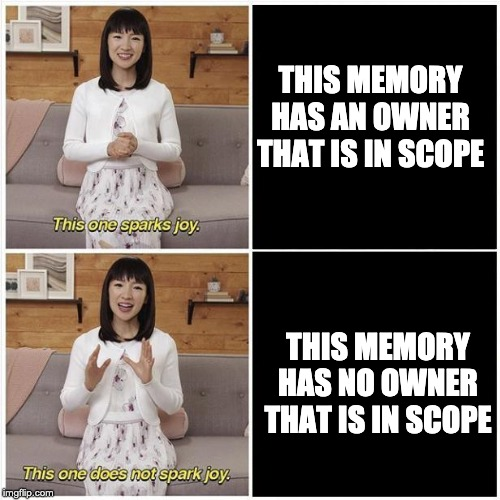
\includegraphics[width=0.7\textwidth]{images/joy.jpeg}
\end{center}


\end{frame}



\begin{frame}[fragile]
\frametitle{Standard Scope}

Variable scopes are fairly standard.
\begin{lstlisting}[language=Rust]
  fn main() {
    println!("start");
    { // no s
      let s = "I am s";
      println!("s is {}", s);
    } // s now out of scope
  }
\end{lstlisting}

 String objects contain a heap component,
which may be allocated and freed.

What can go wrong with heap allocation?

\end{frame}


\begin{frame}[fragile]
\frametitle{It's Yours!}

If you own something, you can change it.

\begin{lstlisting}[language=Rust]
  fn main() {
    let s = String::from("hello"); // immutable String
    let mut s2 = String::from("459 assignments"); // mutable String
    s2.push_str(", maybe?");
    println!("got string {}", s);
  }
\end{lstlisting}

\end{frame}


\begin{frame}[fragile]
\frametitle{Time to Die?}

Rust uses rule \#3: if something goes out of scope, then drop (free) it.
This is quite like \CPP~RAII (Resource Acquisition is Initialization).

Still, we need a solution for objects that live beyond their original scope, e.g.
return values.
\begin{lstlisting}[language=Rust]
  fn return_a_string() -> String {
    let s = String::from("longevity");
    return s; // transfers ownership (moves) to caller
  }

  fn main() {
    let returned_string = return_a_string();
    println!("string {}", returned_string);
  }
\end{lstlisting}

Ownership is transferred...

\end{frame}


\begin{frame}[fragile]
\frametitle{Transferring Ownership}

\begin{lstlisting}[language=Rust]
  let s1 = String::from("no surprise");
  println!("can print {}", s1);
  let s2 = s1;
  println!("can still print {}", s2);
  println!("this line won't compile! {}", s1); // no longer owns
\end{lstlisting}

(Stack variables are copied.)

\end{frame}


\begin{frame}
\frametitle{Well, you see...}

Rust strings are a hybrid, containing both a stack part and a heap part.

\begin{center}
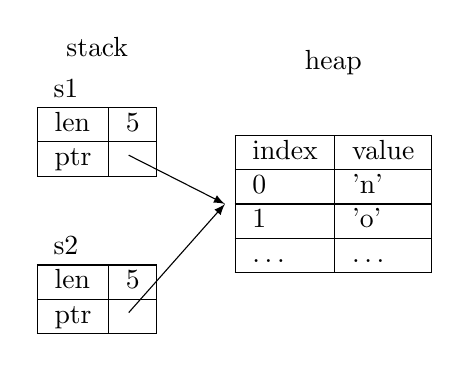
\begin{tikzpicture}
\draw (0,1) node {stack};
\draw (0,0) node (one) {
\begin{tabular}{|l|l|}
\multicolumn{2}{l}{s1} \\
\hline
len & 5 \\ \hline
ptr & \\ \hline
\end{tabular}
};

\draw (0,-2) node (two) {
\begin{tabular}{|l|l|} 
\multicolumn{2}{l}{s2} \\ \hline
len & 5 \\ \hline
ptr & \\ \hline
\end{tabular}
};

\draw (3,0.8) node {heap};
\draw (3, -1) node (s) {
\begin{tabular}{|l|l|} \hline
index & value \\ \hline
0 & 'n' \\ \hline
1 & 'o' \\ \hline
\ldots & \ldots \\ \hline
\end{tabular}
};

\path[draw,-{latex}] (one) ++ (0.4,-0.38) -- (s.west);
\path[draw,-{latex}] (two) ++ (0.4,-0.38) -- (s.west);

\end{tikzpicture}
\end{center}

The assignment {\tt let s2 = s1} carries out a shallow copy of the stack part. Rust
does not automatically copy the heap part.

What should get freed?

\end{frame}



\begin{frame}
\frametitle{It's Yours Now}

After the move, {\tt s1} is no longer valid.


Ownership of the heap part is moved from {\tt s1} to {\tt s2} by the assignment.

Only when {\tt s2} goes out of scope do we free the heap object.


And because the heap object only has one owner, it is only freed once.

Deep copy is possible with ``clone'', if used explicitly.

\end{frame}


\begin{frame}[fragile]
\frametitle{Take It!}


Move semantics also applies to function calls and return values, e.g.
\begin{lstlisting}[language=Rust]
  fn main() {
    let s = String::from("moving to callee");
    callee(s); // afterwards, s is invalid
  }
  fn callee(param:String) {
    println!("got {}, param");
  } // param goes out of scope, object dropped
\end{lstlisting}

If you return something, then the ownership passes back to the caller.


\end{frame}



\begin{frame}[fragile]
\frametitle{Borrowing}

\begin{center}
	
\includegraphics[width=0.4\textwidth]{images/steve.jpeg}
\end{center}


\begin{lstlisting}[language=Rust]
  fn main() {
    let s = String::from("459");
    let len = calculate_length(s);
    println!("string {} has length {}", s /* we still have it! */,
             len);
  }
  fn calculate_length(s:&String) -> usize { // note the & for borrow
    s.len() // last expr is return value
  } // s is ref so nothing goes out of scope
\end{lstlisting}


\end{frame}

\begin{frame}[fragile]
\frametitle{References and Borrowing}

 Like other variables, references are immutable by default.
We can have mutable references, though.
\begin{lstlisting}[language=Rust]
  fn change(s:&mut String) {
    s.push_str("more");
  }
  fn main() {
    let mut main_str = String::from("some ");
    change(&mut main_str); // create mutable ref to main_str
  }
\end{lstlisting}


\end{frame}

\begin{frame}[fragile]
\frametitle{One Change Only}

The following code won't compile:
\begin{lstlisting}[language=Rust]
  let mut s = String::from("one");
  let r1 = &mut s;
  let r2 = &mut s; // rustc complains!
\end{lstlisting}
In fact, while {\tt r1} is in scope, you can't do anything with the original {\tt s}.
The only way to access the string is through {\tt r1}. Once {\tt r1} goes out of scope,
you can create {\tt r2}.

Since there is only one way to access {\tt r1}, then there will be no race conditions.

\end{frame}

\begin{frame}[fragile]
\frametitle{Immutable Refs}

This is OK:
\begin{lstlisting}[language=Rust]
  let mut s = String::from("one");
  let r1 = &s;
  let r2 = &s; // no problem!
\end{lstlisting}
But you can't then do {\tt let r3 = \&mut s;}.

You can have as many outstanding immutable refs as you want.
If there are any immutable refs, you can't have \alert{any} mutable refs. The immutable
refs must go out of scope first.

\end{frame}


\begin{frame}[fragile]
\frametitle{Use after Free}

You also can't commit use-after-free errors: you can't return a ref that outlives
its value.
\begin{lstlisting}[language=Rust]
  fn dangle() -> &String {
    let s = String::from("hello");
    &s // rustc complains: s goes out of scope with active refs
  }
\end{lstlisting}

Rust also has \alert{smart pointers}, which may be reference counted. 

\end{frame}


\begin{frame}
\frametitle{Fearless Concurrency}
\begin{center}
	
\includegraphics[width=0.6\textwidth]{images/mindkiller.jpeg}
\end{center}

As with many other aspects of Rust, we trade compiler errors for runtime
errors; in this case, runtime concurrency errors like race conditions.


That is, the type system ensures concurrency safety!

\end{frame}


\begin{frame}[fragile]
\frametitle{We know what to do}

Rust uses a fork/join model like pthreads. It delegates to the operating
system's threads support and hence implements 1:1 threads.
\begin{lstlisting}[language=Rust]
  let handle = thread::spawn(|| { // closure (can put args between ||)
    // thread code goes here
  });
  // main thread continues here
  handle.join.unwrap(); // unwrap: panic in case of error
\end{lstlisting}
This is not too different from \CPP.


\end{frame}


\begin{frame}[fragile]
\frametitle{Your Data. Give them to me.}

OK, how do we share data between threads? We can move it from main to thread:
\begin{lstlisting}[language=Rust]
  let v = vec![1,2,3];
  let handle = thread::spawn(move || { // move: everything accessed inside closure is moved
    println!("vector {:?}", v);
  }); // no longer have access to v in main
  handle.join().unwrap();
\end{lstlisting}
Rust is saving you from being able to concurrently access {\tt v} in main and thread.


\end{frame}


\begin{frame}[fragile]
\frametitle{Message Passing}

In this case, each value still only has one owner. 

We use \alert{channels}. 

The ownership passes
from the sender, through the channel, to the receiver.
\begin{lstlisting}[language=Rust]
  use std::thread;
  use std::sync::mpsc; // multi producer, single consumer

  fn main() {
    let (tx, rx) = mpsc::channel(); // tx is cloneable
    thread::spawn(move || { // here, tx goes to closure
      let val = String::from("april");
      tx.send(val).unwrap(); // val moved from sender
    });
    let received = rx.recv().unwrap();
    println!("got: {}", received);
  }
\end{lstlisting}
Note the send/receive pair. There is also {\tt try\_recv} to do nonblocking receives.


\end{frame}


\begin{frame}[fragile]
\frametitle{No Escape from Sharing}

We'll need to talk about multiple ownership. But let's talk about mutexes first.
\begin{lstlisting}[language=Rust]
  use std::sync::Mutex;
  fn main() {
    let m = Mutex::new(5); // mutex guards access to an i32
    {
      let mut num = m.lock().unwrap();
      // unwrap: maybe some other thread panicked while holding lock;
      //         then we panic too.
      *num = 6; // "deref" the mutex (is actually a smart pointer)
    } // release lock when num goes out of scope
    println!("m={:?}", m);
  }
\end{lstlisting}
Well, that's fine, but it's just one thread. We really do need multiple ownership
to share data.

\end{frame}


\begin{frame}[fragile]
\frametitle{Count... Again?}

 The shared data needs to be owned by all threads, and a naive solution
will get rejected by the borrow checker. 

Instead, we have to use \alert{reference counted
  cells}, implemented by {\tt Arc}.
% end of 3rd lecture
\begin{lstlisting}[language=Rust]
  use std::sync::{Mutex, Arc};
  use std::thread;
  fn main() {
    let counter = Arc::new(Mutex::new(0)); // atomic reference cell
    let mut handles = vec![];

    for _ in 0..10 {
      let counter = Arc::clone(&counter); // clone the Arc
      let handle = thread::spawn(move || {
        let mut num = counter.lock().unwrap();
        *num += 1;
      });
      handles.push(handle);
    }
    for handle in handles {
      handle.join().unwrap();
    }
    println!("result: {}", *counter.lock().unwrap());
  }
\end{lstlisting}

\end{frame}


\begin{frame}
\frametitle{Lock Ownership}

Rust guarantees that you have the appropriate lock, using ownership (possibly multiple ownership).


Rust does not guarantee lack of deadlocks.


\end{frame}




\end{document}

